\graphicspath{Figures/sus13009}

\chapter{Results and Interpretation}
\label{chap:sus13009results}

\chapterquote{In fact, the mere act of opening the box will determine the state of the
cat, although in this case there were three determinate states the cat
could be in: these being Alive, Dead, and Bloody Furious.}
{Terry Pratchett, 1948 -- 2015: Lords and Ladies}


In this chapter, we show the results and interpretations of a search for events containing a single energetic jet and missing transverse momentum, 
using a data sample collected at 8~\TeV by the \ac{CMS} detector at the \ac{CERN} \ac{LHC} and corresponding to an integrated luminosity of 19.7~\fbinv.
The search described in Chapter~\ref{chap:sus13009} is interpreted in the context of \ac{SMS} of \ac{SUSY} in the third generation.


\section{Results}
A summary of the predictions and corresponding uncertainties for all the \ac{SM} backgrounds, as discussed in Section~\ref{sec:BKG} is listed in Table~\ref{tab:summary_bgd}, and compared to the data in the search regions.
The distributions of \METmu and $\pt(\jet_1)$ in data as compared to SM predictions in simulation are shown in Figure~\ref{fig:ANA_MET_plots}.
No significant deviation from the \ac{SM} is observed.


\begin{table*}%[!Hhtb]  %table 8   110811:05  
        \begin{center}
\caption{Event yields for the seven inclusive search regions detailed in Chapter~\ref{chap:sus13009}. The \ac{SM} background predictions and the data yields correspond to an integrated luminosity of 19.7~\fbinv and the quoted uncertainties reflect the statistical and systematic contributions.}
\label{tab:summary_bgd}
\footnotesize
                \begin{tabular}{l|lllllll} \hline
$\pt(\,\mathrm{j}_1)$ (\GeV)   &  $> 250$ &   $> 300$ &  $> 350$ &  $> 400$ &  $> 450$ &  $> 500$ &  $> 550$  \\ \hline
\znunu\,+\,jets&21209$\pm$1115  & 10077$\pm$592   & 4597$\pm$324  & 2250$\pm$197  & 1250$\pm$137  & 663$\pm$94    & 334$\pm$65 \\  
W\,+\,jets                            &12328$\pm$707   & 5939$\pm$366    & 2690$\pm$180  & 1246$\pm$92   & 627$\pm$52    & 301$\pm$29    & 150$\pm$18 \\ 
\ttbar                            &602$\pm$301     & 344$\pm$172     & 178$\pm$89    & 91$\pm$46     & 48$\pm$24     & 27$\pm$14     & 18$\pm$9.0 \\
\zellell\,+\,jets    &127$\pm$64      & 75$\pm$38       & 40$\pm$20     & 25$\pm$13     & 17$\pm$8.3    & 11$\pm$5.6    & 7.4$\pm$3.7\\
Single top                          &172$\pm$86      & 97$\pm$49       & 49$\pm$24     & 21$\pm$10     & 11$\pm$5.7    & 5.2$\pm$2.6   & 3.2$\pm$1.6\\
QCD Multijets                     &786$\pm$473     & 508$\pm$306     & 304$\pm$184   & 162$\pm$99    & 80$\pm$49     & 52$\pm$32     & 28$\pm$18  \\
Diboson                           &639$\pm$320     & 369$\pm$184     & 206$\pm$103   & 113$\pm$56    & 64$\pm$32     & 36$\pm$18     & 21$\pm$10  \\ \hline
Total SM                          &35862$\pm$1474  & 17409$\pm$803   & 8064$\pm$437  & 3907$\pm$250  & 2098$\pm$160  & 1096$\pm$106  & 563$\pm$71 \\
Data                              &36582           & 17646           & 8119          & 3896          & 1898          & 1003          & 565        \\ \hline

       \end{tabular}                                                                                   
\end{center}
\end{table*}



\begin{figure}[ht!]
  \begin{center}
  \includegraphics[scale=0.39]{Figures/sus13009/MetLep1mu.pdf}
   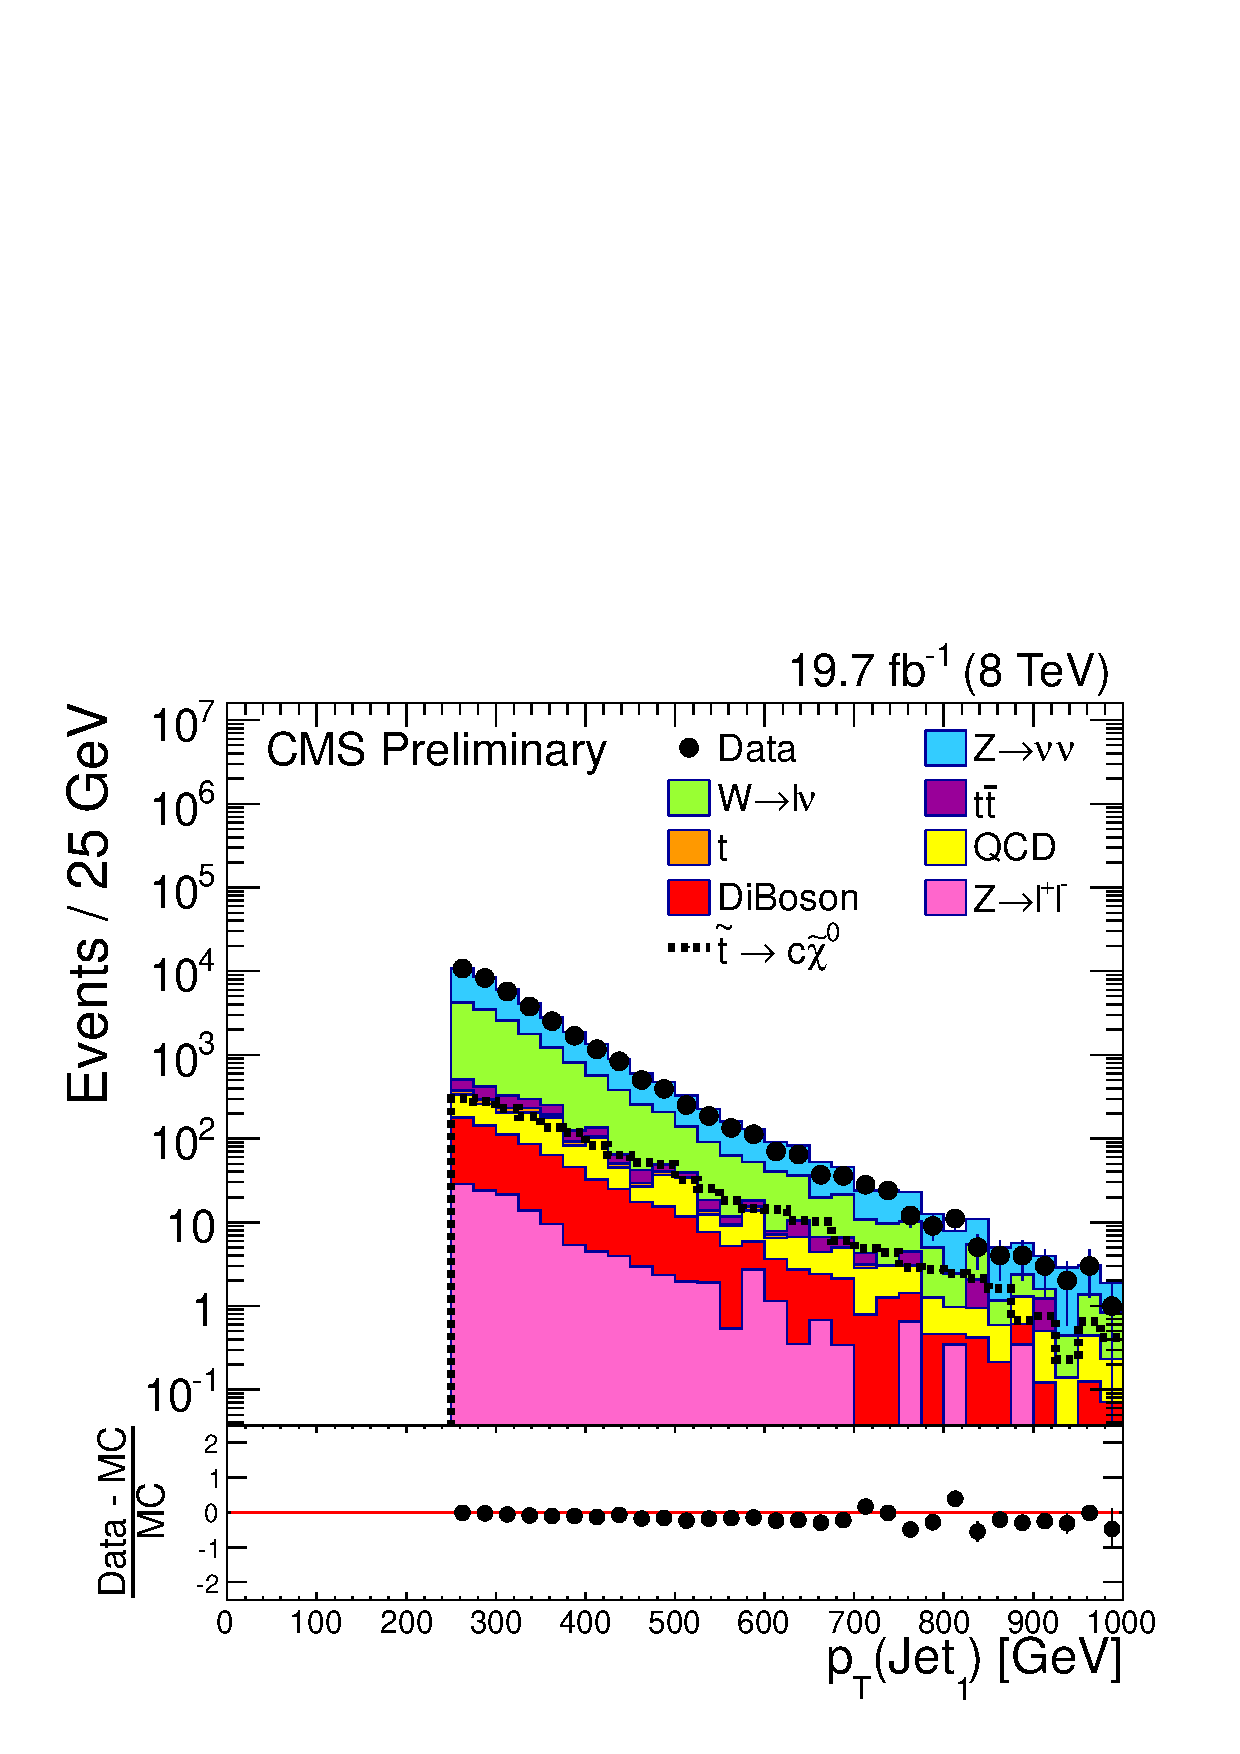
\includegraphics[scale=0.39]{Figures/sus13009/Jet1Pt.pdf}
  \caption{Distributions of (left) \METmu and (right) leading jet $\pt$ in the baseline monojet search region, $\pt(\jet_1) > 250$~\GeV, for data and SM backgrounds. Background distributions are taken from simulation, and normalized to an integrated luminosity of 19.7~\fbinv. A representative signal distribution for $\sTop \rightarrow \mathrm{c} \chiOneZero$ is also shown (in the dotted line), where $m_{\sTop} = 250~\GeV$ and $m_{\chiOneZero} = 240~\GeV$.  Statistical uncertainties are shown for the data.
  Taken from Ref.~\cite{sus14001}.
\label{fig:ANA_MET_plots}}
  \end{center}
\end{figure}


%
\section{Interpretation} 
\label{sec:GEN}

No significant deviations from the \ac{SM} predictions are observed. 
To interpret the consistency of the observed number of events with
the background expectation in the context of compressed \ac{SUSY}, and also to
enable comparison with previous results, we set limits on the production cross section of top and bottom squarks as a function of the top and bottom squark mass and the LSP mass. 

Simulation of signal events 
$\sTop\rightarrow\charmquark\chiOneZero$ and 
$\sBot\rightarrow\bottomquark\chiOneZero$ is necessary to evaluate the sensitivity of the event selection to the \ac{SMS} models probed, and therefore the compatibility of the results in Table~\ref{tab:summary_bgd} to these signatures of new physics.

\subsection{Simulation of signal events}

Simulation of signal events is in the \ac{SMS}~\cite{bib:SMS} framework as described in Section~\ref{sec:susycolliders}. 
As the monojet event selection relies on an \ac{ISR} jet, the acceptance of signal events is low due to the additional factor of $\alpha_s$ on production cross sections - typically around 1\% of events satisfy selection requirements. 
Therefore, many events are necessary to ensure uncertainties are not dominated by statistical uncertainties. 
In addition, scans consist of many points in the ($m_{\sTop}, m_{\chiOneZero}$) and ($m_{\sBot}, m_{\chiOneZero}$) mass planes in order to give good coverage across the phase space region of interest. 
As a result, millions of events are required and the signal MC simulation samples are huge - for example, the $\sTop \rightarrow \charmquark \chiOneZero$ sample takes up diskspace of order 1~TB.
Generating these samples is then a computational challenge. 
We cannot use a vast number of computing hours, nor wait years for their production. 
So, an alternative method of MC generation has been developed, as compared to the \ac{SM} background samples detailed in Section~\ref{sec:GEN}.

Events are generated using \MADGRAPH{}5 and showered with \PYTHIA{}6.4.24 with up to 2 partons. To speed up the generation process, the CMS detector response is simulated using the CMSSW FastSim prescription~\cite{FASTSIM}. 
It gives an accurate detector response to the physics objects, but takes less than 1/100$^{\rm th}$ of the time that the full \GEANTfour detector simulation takes. 
The rate of production is therefore increased by a factor 100, allowing the large samples necessary to be generated.
The MLM matching prescription~\cite{MLMmatching}, which matches hard partons from the first stage of simulation to jets produced after hadronization, is used to avoid double counting between the matrix element calculations and parton showering.
Top and bottom squark production cross sections are taken from the LHC SUSY Cross Section Working Group~\cite{bib:SUSYxs}.

Top squark signal simulation 
contains events where pair produced top squarks decay via $\sTop\rightarrow\charmquark\chiOneZero$ with 100\% branching fraction
in the ($m_{\sTop}, m_{\sTop} - m_{\chiOneZero}$) mass plane from $m_{\sTop} =$100~\GeV to 350~\GeV in steps of 25~\GeV, and 
$\dmstop = m_{\sTop} - m_{\chiOneZero} = $ 10, 20, 30, 40, 60, and 80~\GeV. 
There are two additional points at  $m_{\sTop} =$250, 275~\GeV and $\dmstop = $ 5 to probe the monojet limit towards top squark-LSP degeneracy.
An additional set of events at $m_{\sTop} =$ 200~\GeV and $m_{\sTop} - m_{\chiOneZero} =$ 10, 80~\GeV were showered with up to 3 partons.



Bottom squark signal simulation 
contains events where pair produced bottom squarks decay via $\sBot\rightarrow\bottomquark\chiOneZero$ with 100\% branching fraction
in the ($m_{\sBot}, m_{\chiOneZero}$) mass plane.
The scan is less granular, and covers a wider phase space range: 
$m_{\sBot} =$100~\GeV to 450~\GeV in steps of 25~\GeV, and 
$m_{\chiOneZero} = $ 1, 50, 100...~\GeV, for $m_{\chiOneZero} < m_{\sBot}$.
There are also points generated close to the degeneracy line, at 
$\dmsbot = m_{\sBot} - m_{\chiOneZero} = 10$~\GeV.


\section{Signal acceptance}

Here, we refer to signal acceptance as the kinetic acceptance of the signal multiplied by the efficiency of reconstruction. 

The signal acceptance in the search regions is calculated for each mass point. 
Results for the \sTop signal are shown in Figure~\ref{fig:stopAcc}, for a selection of representative values of $m_{\sTop}$.
As expected, those signal points which have the smallest mass difference \dmstop have the greatest signal acceptances, as these look most like a true monojet event. 
Signal acceptance also increases with $m_{\sTop}$.
Here, the mass difference $\dmstop$ never exceeds 80~\GeV.


\begin{figure}[ht!]
  \begin{center}
  \includegraphics[scale=0.35]{Figures/sus13009/limitplots/plots/stop/acceptance_100.pdf}
  \includegraphics[scale=0.35]{Figures/sus13009/limitplots/plots/stop/acceptance_150.pdf}
  \includegraphics[scale=0.35]{Figures/sus13009/limitplots/plots/stop/acceptance_200.pdf} 
  \includegraphics[scale=0.35]{Figures/sus13009/limitplots/plots/stop/acceptance_250.pdf}
  \includegraphics[scale=0.35]{Figures/sus13009/limitplots/plots/stop/acceptance_300.pdf} 
  \includegraphics[scale=0.35]{Figures/sus13009/limitplots/plots/stop/acceptance_350.pdf}   
   
  \caption{Signal acceptances in the search regions, at each $\pt(\jet_1)$ threshold for the process \ttwocc. Each plot shows a different value of $m_{\sTop}$, and various masses of the LSP, $m_{\chiOneZero}$. Signal acceptance is greatest when $m_{\sTop}$ is close to $m_{\chiOneZero}$, and increases with increasing $m_{\sTop}$.
\label{fig:stopAcc}}
  \end{center}
\end{figure}


The signal acceptance in the search regions for the \sBot signal are shown in Figure~\ref{fig:sbottomAcc}.
For the compressed regions, where $\dmsbot\leq100~\GeV$, we observe a similar behaviour to that seen in Figure~\ref{fig:stopAcc}.
The lower granularity of this signal compared to the \ttwocc signal is evident as there are less values of $m_{\chiOneZero}$ for each $m_{\sBot}$ in the compressed regions. 
There are also signal points for $\dmsbot > 80~\GeV$, and for low values of $m_{\chiOneZero}$, we observe relatively high signal acceptances for the lower jet threshold search regions, which then decreases at higher thresholds.
Lower numbers of events in the simulation for the mass points for which $\dmsbot\geq 150~\GeV$ is apparent, as the acceptance varies more with increasing $\pt(\jet_1)$.


\begin{figure}[ht!]
  \begin{center}
  \includegraphics[scale=0.35]{Figures/sus13009/limitplots/plots/sbottom/acceptance_100.pdf}
  \includegraphics[scale=0.35]{Figures/sus13009/limitplots/plots/sbottom/acceptance_150.pdf}
  \includegraphics[scale=0.35]{Figures/sus13009/limitplots/plots/sbottom/acceptance_250.pdf}
  \includegraphics[scale=0.35]{Figures/sus13009/limitplots/plots/sbottom/acceptance_300.pdf} 
  \includegraphics[scale=0.35]{Figures/sus13009/limitplots/plots/sbottom/acceptance_350.pdf} 
  \includegraphics[scale=0.35]{Figures/sus13009/limitplots/plots/sbottom/acceptance_400.pdf}     
  \caption{Signal acceptances in the search regions, at each $\pt(\jet_1)$ threshold for the process \ttwobb. Each plot shows a different value of $m_{\sBot}$, and various masses of the LSP, $m_{\chiOneZero}$. Signal acceptance is greatest when $m_{\sBot}$ is close to $m_{\chiOneZero}$, and increases with increasing $m_{\sTop}$.
\label{fig:sbottomAcc}}
  \end{center}
\end{figure}


Signal acceptances of some representative mass hypothesis for \ttwocc and \ttwobb signals are shown in Table~\ref{tab:mono_sigAcc} along with their statistical uncertainties. 



\newsavebox{\Boxa}
\begin{table}[h]
\small
      %  \fontsize{10 pt}{1.2 em}
        \begin{center}
        \caption{\label{tab:mono_sigAcc} Signal acceptance $\times$ efficiency, shown in \%, for each step of the event selection. 
        Two representative mass points are shown; ($m_{\sBot}$, $m_{\chiOneZero}$) = (250,240) and (150,50)~\GeV for $\ttwobb$ where $\mathcal{B}(\sBot\rightarrow\bottomquark\chiOneZero)$ = 1.0, 
        and ($m_{\sTop}$, $m_{\chiOneZero}$) = (250,240)~\GeV and (200,120) for $\ttwocc$, where $\mathcal{B}(\sTop\rightarrow\charmquark\chiOneZero)$ = 1.0.
        Only statistical uncertainties are shown.}
         \begin{lrbox}{\Boxa}
        \begin{tabular}{|l||c|c||c|c|} 
        \hline

\multirow{3}{*}{Monojet event selection } & \multicolumn{2}{c||}{$\ttwobb$} & \multicolumn{2}{c|}{$\ttwocc$} \\[0.5ex] \cline{2-5}
 & \multicolumn{2}{c||}{ $\mathcal{B}(\sBot\rightarrow\bottomquark\chiOneZero)$ = 1.0 } & \multicolumn{2}{c|}{ $\mathcal{B}(\sTop\rightarrow\charmquark\chiOneZero)$ = 1.0 }\\[0.5ex]\cline{2-5} 

 %&\multicolumn{2}{c}{  $\ttwobb$ ; $\mathcal{B}(\sbottom\rightarrow\bottomquark\chiOneZero) = 1.0$ } &\multicolumn{2}{c}{  $\ttwocc$ ; $\mathcal{B}(\sTop\rightarrow\rm{c}\chiOneZero) = 1.0$ } \\ [0.5ex]\hline

 & (250, 240)~\GeV & (150, 50)~\GeV& (250, 240)~\GeV & (200, 120)~\GeV   \\ [0.5ex]\hline

Event cleaning                     &   98.61 $\pm$   0.24 &   98.79 $\pm$  0.02 &   97.54 $\pm$   0.14  &   99.21 $\pm$  0.03 \\  
$\MET >$~200~\GeV               &   7.41 $\pm$   0.49  &   2.37 $\pm$  0.02  &    7.17 $\pm$   0.25  &    4.29 $\pm$  0.06 \\  
Noisy events                    &   6.90 $\pm$   0.47  &   2.22 $\pm$  0.02  &    6.68 $\pm$   0.24  &    4.01 $\pm$  0.06 \\  
$\pt(\jet_1)>110$~\GeV          &   6.58 $\pm$   0.46  &   2.08 $\pm$  0.02  &    6.35 $\pm$   0.23  &    3.71 $\pm$  0.06 \\  
$\njets<3$                     &   5.78 $\pm$   0.44  &   1.39 $\pm$  0.02  &    5.56 $\pm$   0.22  &    2.30 $\pm$  0.04 \\  
$\Delta \phi(\jet_1,\jet_2)<2.5$&   5.58 $\pm$   0.43  &   1.170 $\pm$  0.015  &    5.36 $\pm$   0.21  &    1.96 $\pm$  0.04 \\  
$\mu$ veto                      &   5.57 $\pm$   0.43  &   1.170 $\pm$  0.015  &    5.36 $\pm$   0.21  &    1.96 $\pm$  0.04 \\  
$\e$ veto                        &   5.57 $\pm$   0.43  &   1.160 $\pm$  0.015  &    5.36 $\pm$   0.21  &    1.96 $\pm$  0.04 \\  
$\tauh$ veto                 &   5.52 $\pm$   0.43  &   1.14 $\pm$  0.015  &    5.30 $\pm$   0.21  &    1.93 $\pm$  0.04 \\
\hline  
\MET \& $\pt(\jet_1) > 250$~\GeV&   2.08 $\pm$   0.27  &  0.222 $\pm$ 0.006  &    2.04 $\pm$   0.13  &    0.42 $\pm$  0.02 \\  
$\pt(\jet_1) > 300$~\GeV        &   1.32 $\pm$   0.21  &  0.122 $\pm$ 0.005  &    1.32 $\pm$   0.11  &    0.25 $\pm$  0.01 \\  
$\pt(\jet_1) > 350$~\GeV        &   0.80 $\pm$   0.17  &  0.058 $\pm$ 0.003  &    0.81 $\pm$  0.08  &    0.13 $\pm$  0.01 \\  
$\pt(\jet_1) > 400$~\GeV        &   0.49 $\pm$   0.13  &  0.027 $\pm$ 0.002  &    0.50 $\pm$  0.07  &   0.072 $\pm$ 0.008 \\  
$\pt(\jet_1) > 450$~\GeV        &   0.31 $\pm$   0.11  &  0.016 $\pm$ 0.002  &    0.32 $\pm$  0.05  &   0.041 $\pm$ 0.006 \\  
$\pt(\jet_1) > 500$~\GeV        &   0.19 $\pm$  0.08  &  0.009 $\pm$ 0.001  &    0.19 $\pm$  0.04  &   0.023 $\pm$ 0.005 \\  
$\pt(\jet_1) > 550$~\GeV        &   0.12 $\pm$  0.07  &  0.006 $\pm$ 0.001  &    0.12 $\pm$  0.03  &   0.013 $\pm$ 0.003 \\ \hline
\end{tabular}
\end{lrbox}
\scalebox{0.90}{\usebox{\Boxa}}
\end{center}
\end{table}
 




\subsection{Signal acceptance in 2- and 3-parton simulation}

The difference in signal acceptance between the 2-parton and 3-parton samples produced for \ttwocc 
is found to be small; Table~\ref{tab:2_3_partonAcc} lists the acceptances for both samples.
In the signal regions the differences in the acceptance is, at most, 0.04\%, 
and generally it is less where the analysis is most sensitive (for small mass differences).
We conclude the effect of generating 2 or 3 partons with the signal does not have a significant effect on the result.
Nevertheless, the differences are accounted for in the uncertainty on the signal acceptance.

\newsavebox{\Boxb}
\begin{table}[!Hhtb]
\begin{center}
\caption{Acceptances (in \%) of 2-parton and 3-parton samples for mass points ($m_{\sTop}, m_{\chiOneZero}$) = (200,190)~\GeV and (200,120)~\GeV. The modulus of the differences in the acceptances from the two samples are listed. } 
\label{tab:2_3_partonAcc}
\begin{lrbox}{\Boxb}
\begin{tabular}{ l |ccc|ccc} \hline
 \multicolumn{1}{c|}{\multirow{2}{*}{ Event selection}} & \multicolumn{3}{c|}{($m_{\sTop}, m_{\chiOneZero}$) = (200,190)}& \multicolumn{3}{c}{($m_{\sTop}, m_{\chiOneZero}$) = (200,120)} \\ 
    &  2 partons  & 3 partons & $|$Difference$|$ &  2 partons & 3 partons & $|$Difference$|$\\ 
    \hline
Abnormal events         & 97.1  & 97.1  & 0     & 99.3  & 99.19 & 0.11  \\
$\METmu > 200~\GeV$     & 2.74  & 2.61  & 0.13  & 1.84  & 1.79  & 0.05  \\
Noise clean             & 2.58  & 2.47  & 0.11  & 1.75  & 1.71  & 0.04  \\
$\pt(\jet_1)>110~\GeV$  & 12.53 & 2.42  & 0.11  & 1.71  & 1.68  & 0.03  \\
$\njets<3$              & 2.14  & 2.06  & 0.08  & 0.94  & 0.98  & 0.04  \\
$\Delta \phi(\jet_1, \jet_2) <2.5$ &2.05  & 1.99  & 0.06  & 0.78  & 0.79  &  0.01 \\
$\e$ veto               & 2.05  & 1.99  & 0.06  & 0.78  & 0.79  &  0.01 \\
$\mu$ veto              & 2.05  & 1.99  & 0.06  & 0.78  & 0.79  &  0.01 \\
$\tauh$ veto            & 2.02  & 1.97  & 0.05  & 0.77  & 0.77  & 0     \\
$\pt(\,\mathrm{j}_1)>250$~\GeV & \multirow{2}{*}{1.32}
       & \multirow{2}{*}{1.36}   
       & \multirow{2}{*}{0.04}
       & \multirow{2}{*}{0.43}
       & \multirow{2}{*}{0.41}
       & \multirow{2}{*}{0.02}\\
               \,\,\& $\METmu>250$~\GeV   &   &   &   &   &               \\
$\pt(\jet_1)$$>$300~\GeV  & 0.86  & 0.88  &  0.02 & 0.25  & 0.23  & 0.02  \\
$\pt(\jet_1)$$>$350~\GeV  & 0.51  & 0.51  & 0     & 0.14  & 0.12  & 0.02  \\
$\pt(\jet_1)$$>$400~\GeV  & 0.30  & 0.30  & 0     & 0.076 & 0.063 & 0.013 \\
$\pt(\jet_1)$$>$450~\GeV  & 0.17  & 0.18  &  0.01 & 0.042 & 0.025 & 0.017 \\
$\pt(\jet_1)$$>$500~\GeV  & 0.10  & 0.10  & 0     & 0.024 & 0.013 & 0.011 \\
$\pt(\jet_1)$$>$550~\GeV  & 0.067 & 0.056 & 0.011 & 0.014 & 0.006 & 0.008 \\
\hline
\end{tabular}  
\end{lrbox}
\scalebox{0.87}{\usebox{\Boxb}}    
\end{center}
\end{table}


\subsection{Systematic Uncertainties on Signal}
\label{sec:signalSYST}

% The analysis is reliant upon an \ac{ISR} jet, thus the signal modelling of \ac{ISR} is very important.
% This is the dominant source of uncertainty on the signal.

The selection of signal events (and therefore the signal acceptance) in this analysis relies on a high-\pt ISR jet, so the modelling of ISR must be reliable.
The simulated and measured \pt spectra of recoiling systems against ISR jets is studied in Ref.~\cite{CMSsinglelep} for Z\,+\,jets, 
\ttbar and other processes. 
The simulation is found to over predict the data by 20\% for ISR jets with $\pt > 250$ \GeV, see Figure~\ref{fig:ISRsyst}.
All signal acceptances have therefore been weighted by a factor of 0.8 to correct for this difference, and a systematic uncertainty of 20\% is assigned to each search region to account for this difference for the high \pt ISR jets involved.

\begin{figure}[ht!]
  \begin{center}
  \includegraphics[scale=0.35]{Figures/sus13009/ISRmodellingSUS13011.pdf}
  \caption{Taken from~\cite{CMSsinglelep}, the comparison of data to the prediction from simulation of the jet recoil system in \ttbar events. The data/MC ratio, in the top of the figure, shows that for jets $>250~\GeV$, the simulation over predicts the data.
\label{fig:ISRsyst}}
  \end{center}
\end{figure}


Other sources of uncertainty on the signal are considered. They are:
\begin{itemize}
  \item the uncertainty on the \ac{JES}, which is evaluated by taking the difference in acceptances when the jet \ptv is shifted up and down by an $\eta$ and $\pt$ dependent factor. The difference in acceptances between varying the energy scale up and down is less than 1\% in the signal regions: see Table~\ref{tab:JESuncert}. 
  \item uncertainties on the \ac{PDFs}. The PDF uncertainty for a representative signal sample was found to be less than 2$\%$. 
  \item the difference in acceptance that is obtained from generating signal events with up to 3 partons in \MADGRAPH rather than 2 partons ($<1\%$). 
\end{itemize}

The total uncertainty on the signal in each signal region is taken to be a conservative 25$\%$.
The error on the luminosity measurement is 2.6\% ~\cite{lumi:Summer2013}.

\newsavebox{\Boxc}
\begin{table}[!Hhtb]
\begin{center}
\caption{Acceptances (in \%) of signal samples for mass points ($m_{\sTop}, m_{\chiOneZero}$) = (200,190)~\GeV and (200,120)~\GeV, for when the energy scale is increased and decreased. The modulus of the differences in the acceptances from the two samples are listed. } 
\label{tab:JESuncert}
\begin{lrbox}{\Boxc}
\begin{tabular}{ l |ccc|ccc} \hline
 \multicolumn{1}{c|}{\multirow{2}{*}{ Search region}} & \multicolumn{3}{c|}{($m_{\sTop}, m_{\chiOneZero}$) = (200,190)}& \multicolumn{3}{c}{($m_{\sTop}, m_{\chiOneZero}$) = (200,120)} \\ 
    & JES +  & JES - & $|$Difference$|$ &  JES + & JES - & $|$Difference$|$\\ 
   \hline
$\pt(\jet_1)$$>$300~\GeV & 1.33 & 1.33 & $<$0.01 & 0.42 & 0.44 & 0.03    \\
$\pt(\jet_1)$$>$300~\GeV & 0.88 & 0.84 & 0.03    & 0.26 & 0.26 & $<$0.01  \\
$\pt(\jet_1)$$>$300~\GeV & 0.52 & 0.50 & 0.03    & 0.14 & 0.14 & $<$0.01   \\
$\pt(\jet_1)$$>$300~\GeV & 0.30 & 0.29 & 0.01    & 0.07 & 0.08 & $<$0.01  \\
$\pt(\jet_1)$$>$300~\GeV & 0.18 & 0.17 & 0.01    & 0.04 & 0.04 & $<$0.01       \\
$\pt(\jet_1)$$>$300~\GeV & 0.11 & 0.10 & 0.01    & 0.02 & 0.02 & $<$0.01   \\
$\pt(\jet_1)$$>$300~\GeV & 0.07 & 0.06 & $<$0.01 & 0.02 & 0.01 & $<$0.01   \\
\hline
\end{tabular}  
\end{lrbox}
\scalebox{0.97}{\usebox{\Boxc}}    
\end{center}
\end{table}



\section{Exclusion limits}
\label{sec:STAT}

The CL$_{s}$ method is used to estimate the 95\% confidence level (CL) for a signal cross section in a counting experiment~\cite{bib:STAT_RooStats,PDG}.
Given the integrated luminosity, signal acceptance, background expectation and number of observed events (with associated uncertainties),
the 95\% CL upper limit on the signal cross section is calculated.
The theoretical top-squark production cross sections, which are equal to the bottom-squark production cross sections, and $\pm1\sigma_{\rm th}$ bands are taken from a collaboration between the \ac{ATLAS}, \ac{CMS}
and \ac{LPCC} \ac{SUSY} working groups. Theory uncertainties are dominated by PDF uncertainties 
and calculations are detailed in Ref.~\cite{bib:SUSYxs}. 
Cross section values can be found in Ref.~\cite{stopsbottomxs}.  
The 95\% CL exclusion limits on production cross sections are compared to the theoretical expectations in order to set lower limits on the top (bottom) squark and LSP masses in the $m_{\sTop}, m_{\chiOneZero}$ ($m_{\sBot}, m_{\chiOneZero}$) mass plane. 


\begin{figure}[!Ht]
  \begin{center}
  \includegraphics[scale=0.35]{Figures/sus13009/limitplots/plots/stop/expected_100.pdf}
  \includegraphics[scale=0.35]{Figures/sus13009/limitplots/plots/stop/expected_150.pdf}
  \includegraphics[scale=0.35]{Figures/sus13009/limitplots/plots/stop/expected_200.pdf} 
  \includegraphics[scale=0.35]{Figures/sus13009/limitplots/plots/stop/expected_250.pdf}
  \includegraphics[scale=0.35]{Figures/sus13009/limitplots/plots/stop/expected_300.pdf} 
  \includegraphics[scale=0.35]{Figures/sus13009/limitplots/plots/stop/expected_350.pdf}  
  \caption{95\% CL expected limit on top-squark production cross section as a function of $\pt(j_{1})$\GeV (i.e. in each search region). Limits for $m_{\sTop}=100,150,200,250,300$ and 350~\GeV are shown, where each line corresponds to $\dmstop=10,20,30,40,60$ and 80~\GeV.}
  \label{fig:expLimStop}
  \end{center}
\end{figure}

Expected limits, displayed as a function of $\pt(\,\mathrm{j}_1)$ for every signal mass hypothesis for the \ttwocc signal, using the background expectation in each search region,
can be found in Figure~\ref{fig:expLimStop} where each plot shows a particular $m_{\sTop}$. 
Similar plots showing the 95\% CL expected limits for the \ttwobb signal are shown in 
Figure~\ref{fig:expLimSbot}.
The signal region where the best (i.e. lowest) expected limit is found is selected as the optimal region in which to set limits for that mass point.
Limits are generally fairly flat across the phase space range, for those mass points in the compressed region where \dmstop and $\dmsbot \lessapprox 100~\GeV$.
A fluctuation in the number of $Z(\mu\mu)$ events at $\pt(\,\mathrm{j}_1)>450$~\GeV leads to a fluctuation in the total background expectation in this search region. 
To ensure smooth limit curves we have discounted this signal region from the limit setting procedure.
For the curves shown in Figure~\ref{fig:expLimSbot}, we are not able to set a limit on the production section of bottom squarks for some mass points when \dmsbot is large (i.e. not the compressed SUSY models) in the search regions with the highest $\pt(\jet_1)$ thresholds. 
This is because the analysis looses sensitivity due to hard cuts on ISR combined with the jet multiplicity requirements.


\begin{figure}[!Hhtb]
  \begin{center}
  \includegraphics[scale=0.35]{Figures/sus13009/limitplots/plots/sbottom/expected_100.pdf}
  \includegraphics[scale=0.35]{Figures/sus13009/limitplots/plots/sbottom/expected_150.pdf}
  \includegraphics[scale=0.35]{Figures/sus13009/limitplots/plots/sbottom/expected_200.pdf} 
  \includegraphics[scale=0.35]{Figures/sus13009/limitplots/plots/sbottom/expected_250.pdf}
  \includegraphics[scale=0.35]{Figures/sus13009/limitplots/plots/sbottom/expected_300.pdf} 
  \includegraphics[scale=0.35]{Figures/sus13009/limitplots/plots/sbottom/expected_350.pdf} 
  \caption{95\% CL expected limit on bottom-squark production cross section as a function of $\pt(j_{1})$\GeV (i.e. in each search region). Limits for $m_{\sBot}=100,150,200,250,300$ and 350~\GeV are shown, where each line corresponds to a different $m_{\chiOneZero}$.}
  \label{fig:expLimSbot}
  \end{center}
\end{figure}


The temperature plots in Figure~\ref{fig:optimalacc} show the signal acceptance in the search region with the best expected limit for both ($m_{\sTop}, m_{\chiOneZero}$) and ($m_{\sBot}, m_{\chiOneZero}$) mass planes.
The temperature plots in Figure~\ref{fig:optimalExp} show the best expected 95\% CL limit across the phase space range, and Figure~\ref{fig:optimalJ1} shows the search region in which this best expected limit is found.
We see that typically, harder leading jet cuts give the better limits along the diagonal, where events are dominated by ISR. 
Also, for larger $m_{\sTop}$ and $m_{\sBot}$, harder jet thresholds give the better limits, as these events are typically more boosted.   


\begin{figure}[!Hhtb]
  \begin{center}
  \includegraphics[scale=0.39]{Figures/sus13009/limitplots/plots/stop/optimal_stop_acceptance.pdf}
  \includegraphics[scale=0.39]{Figures/sus13009/limitplots/plots/sbottom/optimal_sbottom_acceptance.pdf}
  \caption{The temperature plot shows acceptance of the signal point where the best expected limit is found, across the ($m_{\sTop}, m_{\chiOneZero})$ (left) and ($m_{\sBot},m_{\chiOneZero}$) (right) mass planes.}
  \label{fig:optimalacc}
  \end{center}
\end{figure}

\begin{figure}[!Hhtb]
  \begin{center}
  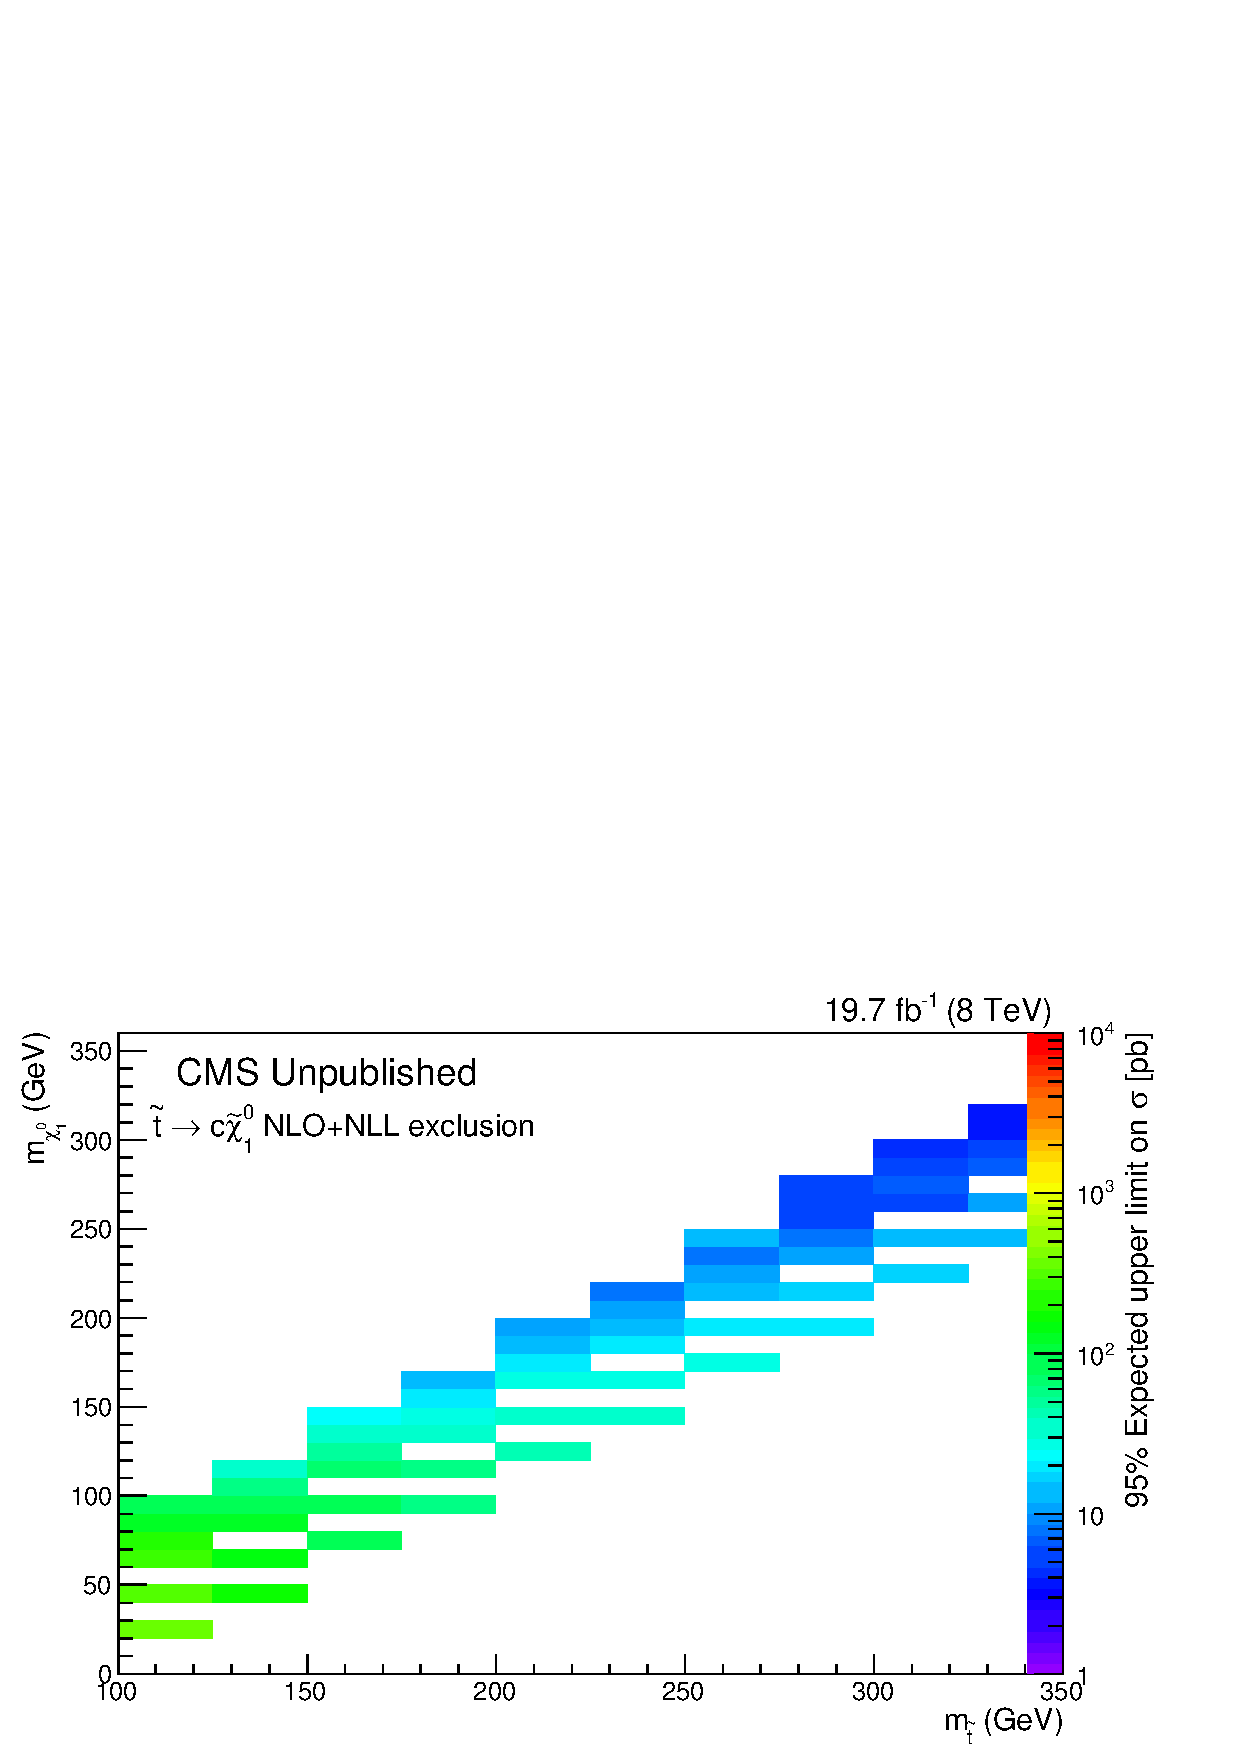
\includegraphics[scale=0.39]{Figures/sus13009/limitplots/plots/stop/optimal_stop_expected.pdf}
  \includegraphics[scale=0.39]{Figures/sus13009/limitplots/plots/sbottom/optimal_sbottom_expected.pdf}
  \caption{The temperature plot shows the best expected limit across the ($m_{\sTop}, m_{\chiOneZero})$ (left) and ($m_{\sBot},m_{\chiOneZero}$) (right) mass planes.}
  \label{fig:optimalExp}
  \end{center}
\end{figure}

\begin{figure}[!Hhtb]
  \begin{center}
  \includegraphics[scale=0.39]{Figures/sus13009/limitplots/optimal_stop_jet1pT.pdf}
  \includegraphics[scale=0.39]{Figures/sus13009/limitplots/optimal_sbottom_jet1pT.pdf}
  \caption{The temperature plot shows search region (the $\pt(\,\mathrm{j}_1)$ threshold) in which the best expected limit is found, across the ($m_{\sTop}, m_{\chiOneZero})$ (left) and ($m_{\sBot},m_{\chiOneZero}$) (right) mass planes. Plots feature in Ref.~\cite{sus14001}.}
  \label{fig:optimalJ1}
  \end{center}
\end{figure}

In the ($m_{\sBot}, m_{\chiOneZero}$) mass plane we also expect sensitivity outside of the compressed region. 
The bottom squark decay $\sBot \rightarrow \bottomquark \chiOneZero$ is valid for mass points that lie outside of similar region in which the top squark decay $\sTop \rightarrow \charmquark \chiOneZero$ dominates, so we are also able to test the sensitivity of the search criteria for signals where $\dmsbot>m_{\W}$.
To understand the signal acceptances outside of the region, we study several mass points for which $m_{\sBot}=225~\GeV$. 
Figure~\ref{fig:sbot225njets} shows the jet multiplicity distributions for $m_{\chiOneZero}=1,50$ and 100~\GeV in the baseline search region where all criteria apart from $\njets<2$ have been applied.  

\begin{figure}[!Hhtb]
  \begin{center}
  \includegraphics[scale=0.39]{Figures/sus13009/Njets_225_Norm.pdf}
  \caption{Normalized distribution of \njets for $\sBot \rightarrow \bottomquark \chiOneZero$ signal points, in the events satisfying the baseline search region criteria, other than $\njets<3$. Signal points are labelled as ($m_{\sBot}, m_{\chiOneZero}$)~\GeV.}
  \label{fig:sbot225njets}
  \end{center}
\end{figure}

%reasons for b-jet limit
As $m_{\chiOneZero}$ decreases, there are fewer events with \njets=1, and more events with higher jet multiplicities. 
This is to be expected, as decay products become harder and a final state single high-\pt jet originating from \ac{ISR} is no longer seen. 
At ($m_{\sBot},m_{\chiOneZero}$) = (225, 100)~\GeV, most events contain one jet. This could be an ISR jet, or similarly a b-jet from the decay of the bottom squark which is energetic enough to pass the $\pt(\jet_1)$ requirement of the baseline signal region.
A significant number of events contain three jets, where the most energetic jet with $\pt>250~\GeV$ is from one of the b-quark decays (or \ac{ISR}), and the two further jets with $\pt>60~\GeV$ are from the second b quark and ISR (or the two b quarks or otherwise). 
These trijet events do not satisfy the requirements of the search region and so acceptance suffers. 
As \dmsbot increases further, at ($m_{\sBot},m_{\chiOneZero}$) = (225, 50)~\GeV, we see most events are classified as having one or two jets. 
Here, the jets are mostly from b quark decay, as both are energetic enough to pass the jet criteria.
Crucially, most of these events will satisfy the search region requirements once $\njets<3$ is applied: the search regions are therefore dijet dominated.
At ($m_{\sBot},m_{\chiOneZero}$)=(225,1)~\GeV we see that more events sit at the higher jet multiplicities. 
We are less dominated by energetic jets from ISR here; instead the \dmsbot is now large enough that b quarks get a significant boost and satisfy $\pt(\jet_1)>250~\GeV$, $\pt(\jet_2)>60~\GeV$. There are more events with softer ISR or FSR jets which push the jet multiplicity up, and reduce the signal acceptance.

Outside of the compressed region, we are then not dominated by \ac{ISR} jets. Optimal signal regions are therefore typically those lower $\pt(\jet_1)$ thresholds, as seen in Figure~\ref{fig:optimalJ1}.
Figure~\ref{fig:jetContent225} shows the origin of jets for the same mass points for events that satisfy the baseline search criteria, including the $\njets<3$ requirement.
The behaviours described above are evident. 

\begin{figure}[!Hhtb]
  \begin{center}
  \includegraphics[scale=0.39]{Figures/sus13009/eventTypes_225.pdf}
  \caption{The topology of events satisfying the baseline search region criteria for ($m_{\sBot}, m_{\chiOneZero}$)=(225,1), (225,50) and (225,100)~\GeV. The origin of the first and second jet in the event is shown for events with one or two jets. Distributions are normalized to unit area.}
  \label{fig:jetContent225}
  \end{center}
\end{figure}

%
Figure~\ref{fig:stop_limits} shows the best 95\% CL expected and observed limits on the top-squark production cross section, 
as a function of the top squark mass for $\dmstop = 10, 20, 30, 40, 60$ and $80~\GeV$.
Figure~\ref{fig:sbottom_10GeV} shows the similar 95\% CL expected and observed limits on the bottom-squark production cross section, 
as a function of the bottom squark mass for $\dmstop = 10$. 
As mass points in the remainder of the bottom squark signal sample are produced in a regular pattern in $(m_{\sBot}, m_{\chiOneZero})$ rather than in $(m_{\sBot}, \dmsbot)$ (as in the \ttwocc case), we show the results for the remainder of $\ttwobb$ phase space in a slightly different plane.
Figure~\ref{fig:sbottom_limits} shows the best expected and observed limits for various bottom squark masses as a function of mass difference, $\dmsbot$.
All plots also show the $\pm1,2 \sigma_{\rm exp}$ bands on the expected limits.




%The results of the monojet search can also be interpreted to constrain the production of light stops. The observed limits on the production cross section as a function of the stop mass are shown in Figure~\ref{fig:stop_limits} for mass splittings of 10 GeV, 30 GeV and 80 GeV. Also shown are the expected limits and the theoretical prediction. The observed (expected) limits on the stop mass for the 10 GeV and 30 GeV mass splitting are; 250 (255) GeV and 190 (195) GeV respectively.
\begin{figure}[!Hhtb]
  \begin{center}
%  \includegraphics[scale=0.39]{m10.pdf}
%  \includegraphics[scale=0.39]{m30.pdf}
%  \includegraphics[scale=0.39]{Figures/sus13009/limitplots/plots/stop/Limit_susy_stop_10.pdf}
%  \includegraphics[scale=0.39]{Figures/sus13009/limitplots/plots/stop/Limit_susy_stop_20.pdf}
%  \includegraphics[scale=0.39]{Figures/sus13009/limitplots/plots/stop/Limit_susy_stop_30.pdf}
%  \includegraphics[scale=0.39]{Figures/sus13009/limitplots/plots/stop/Limit_susy_stop_40.pdf}
%  \includegraphics[scale=0.39]{Figures/sus13009/limitplots/plots/stop/Limit_susy_stop_60.pdf}
%  \includegraphics[scale=0.39]{Figures/sus13009/limitplots/plots/stop/Limit_susy_stop_80.pdf}
  \includegraphics[scale=0.39]{Figures/sus13009/limits//Limit10.pdf}
  \includegraphics[scale=0.39]{Figures/sus13009/limits//Limit20.pdf}
  \includegraphics[scale=0.39]{Figures/sus13009/limits//Limit30.pdf}
  \includegraphics[scale=0.39]{Figures/sus13009/limits//Limit40.pdf}
  \includegraphics[scale=0.39]{Figures/sus13009/limits//Limit60.pdf}
  \includegraphics[scale=0.39]{Figures/sus13009/limits//Limit80.pdf}
  \caption{95\% CL observed and expected limits on the top-squark production cross section as a function of the $m_{\sTop}$ for $m_{\sTop} - m_{\chiOneZero} = 10, 20, 30, 40, 60$ and 80 \GeV. Curves taken from Ref.~\cite{sus13009}.}
  \label{fig:stop_limits}
  \end{center}
\end{figure}

The observed behaviour in Figure~\ref{fig:sbottom_limits} where sbottom quark limits are low for the compressed region, at low $\dmsbot$, increase, and then decrease again for larger \dmsbot is due to the migration of events between bins in jet multiplicity, as described above. 
The signal topology and search region jet requirements means monojet events, dijet events, and higher jet multiplicities dominate in the different regions of phase space and signal acceptance (and hence limits) respond accordingly. 

 % The limits at low mass difference are due to monojet events, 
 %  where an event with a radiated ISR jet passes the event selection. 
 %  At large mass differences, we become sensitive to dijet events; events in which two b-jets from both bottom squark decays pass the event selection.

\begin{figure}[!Hhtb]
  \begin{center}
%  \includegraphics[scale=0.39]{m10.pdf}
%  \includegraphics[scale=0.39]{m30.pdf}
  \includegraphics[scale=0.39]{Figures/sus13009/limitplots/plots/sbottom/Limit_susy_sbottom_10.pdf}
  \caption{95\% CL observed and expected limits on the bottom-squark production cross section as a function of $m_{\sBot}$ for $m_{\sBot} - m_{\chiOneZero} = 10~\GeV$.}
  \label{fig:sbottom_10GeV}
  \end{center}
\end{figure}

\begin{figure}[!Hhtb]
  \begin{center}
  \includegraphics[scale=0.39]{Figures/sus13009/limitplots/plots/sbottom/Limit_DM_sbottom_100.pdf}
  \includegraphics[scale=0.39]{Figures/sus13009/limitplots/plots/sbottom/Limit_DM_sbottom_150.pdf}
  \includegraphics[scale=0.39]{Figures/sus13009/limitplots/plots/sbottom/Limit_DM_sbottom_175.pdf}
  \includegraphics[scale=0.39]{Figures/sus13009/limitplots/plots/sbottom/Limit_DM_sbottom_200.pdf}
  \includegraphics[scale=0.39]{Figures/sus13009/limitplots/plots/sbottom/Limit_DM_sbottom_225.pdf}
  \includegraphics[scale=0.39]{Figures/sus13009/limitplots/plots/sbottom/Limit_DM_sbottom_250.pdf}
  \includegraphics[scale=0.39]{Figures/sus13009/limitplots/plots/sbottom/Limit_DM_sbottom_275.pdf}
    \includegraphics[scale=0.39]{Figures/sus13009/limitplots/plots/sbottom/Limit_DM_sbottom_300.pdf}
  \caption{95\% CL observed and expected limits on the bottom-squark production cross section as a function of the mass difference $m_{\sBot} - m_{\chiOneZero}$, shown for $m_{\sBot} = 100, 150, 175, 200, 225,$ and 275~\GeV. 
  Also shown are the $\pm 1, 2 \sigma_{\rm exp}$ limits. 
 }
  \label{fig:sbottom_limits}
  \end{center}
\end{figure}




Masses where the observed (expected) limits lie beneath the theory cross section we observe (expect) to exclude.
By finding the point of intersection between the observed (expected) and theoretical cross sections, we find the observed (expected) lower limit on the mass of the top or bottom squark for a particular value of $m_{\chiOneZero}$.
Similarly, by finding the intersection between the observed ($\pm 1 \sigma_{\rm exp}$) and $\pm 1 \sigma_{\rm th}$ (theoretical) limits on cross sections, we find the $\pm 1 \sigma_{\rm th}$ ( $\pm 1  \sigma_{\rm exp}$) lower limits on masses.
By doing this for every mass point available we build a contour in the ($m_{\sTop},m_{\chiOneZero}$) and ($m_{\sBot},m_{\chiOneZero}$) mass planes.

Figure~\ref{fig:stop_limits_2D} shows 95\% CL expected $\pm 1 \sigma_{\rm exp}$ and observed limits $\pm 1 \sigma_{\rm th}$ in the ($m_{\sTop},m_{\chiOneZero}$) mass plane assuming 100\% branching fraction to the top squark decay $\sTop \rightarrow \charmquark \chiOneZero$.
Also shown are previous results from the Tevatron.
We are able to exclude the region above a line which goes from approximately $m_{\sTop}=130~\GeV, m_{\chiOneZero}=50~\GeV$ to $m_{\sTop}=260~\GeV, m_{\chiOneZero}=255~\GeV$.  
Because the analysis is insensitive to the final state decay products, we are able to exclude \ttwocc production for $m_{\sTop} \leq 260~\GeV$ and $\dmstop \leq 10~\GeV$: right up to the degeneracy limit. 

Similarly, Figure~\ref{fig:sbottom_limits_2D} shows the 95\% CL expected $\pm 1 \sigma_{\rm exp}$ and observed limits $\pm 1 \sigma_{\rm th}$ in the ($m_{\sBot},m_{\chiOneZero}$) mass plane assuming 100\% branching fraction to bottom squark decay $\sBot \rightarrow \bottomquark \chiOneZero$.
We are able to exclude the region above a line which goes from approximately $m_{\sBot}=140~\GeV, m_{\chiOneZero}=50~\GeV$ to $m_{\sBot}=270~\GeV, m_{\chiOneZero}=265~\GeV$.  
Further, the region where $m_{\sBot} < 165~\GeV$ is excluded for all $m_{\chiOneZero}$.
We also exclude a region at lower $m_{\chiOneZero}$ from approximately $m_{\sBot}=150~\GeV, m_{\chiOneZero}=40~\GeV$ to $m_{\sBot}=275~\GeV, m_{\chiOneZero}=60~\GeV$, above the line extending from $m_{\sBot}=175~\GeV, m_{\chiOneZero}=0~\GeV$ to $m_{\sBot}=275~\GeV, m_{\chiOneZero}=40~\GeV$.
The limit in the compressed region echoes that from the ($m_{\sTop},m_{\chiOneZero}$) mass plane: monojet-like events dominate, and sensitivity to events in the region of the mass plane where decay products are very soft is achieved. 
In the region $\dmsbot>m_{\W}$, we are set limits on $m_{\sBot}$ outside the compressed region. The bottom squark decay products are much more energetic, and dijet events, where both events are both b decay, dominate. 



\begin{figure}[!Hhtb]
  \begin{center}
%  \includegraphics[scale=0.39]{m10.pdf}
%  \includegraphics[scale=0.39]{m30.pdf}
  \includegraphics[scale=0.39]{Figures/sus13009/limits/limits_stopLSP.pdf}
%  \includegraphics[scale=0.39]{Figures/sus13009/limits/limits_stopDM.pdf}
  \caption{ Expected and observed 95\% CL exclusion limits in the ($m_{\sTop}, m_{\chiOneZero}$) mass plane for top-squark pair production, assuming 100\% branching fraction to the decay $\sTop \rightarrow \charmquark \chiOneZero$. The $\pm1\sigma_{exp}$ and $\pm1\sigma_{th}$ curves are also shown. The diagonal grey lines mark the borders of the kinematic regimes surrounding the compressed region of phase space. 
  Taken from Ref.~\cite{sus13009}.}
  \label{fig:stop_limits_2D}
  \end{center}
\end{figure}


\begin{figure}[!Hhtb]
  \begin{center}
  \includegraphics[scale=0.39]{Figures/sus13009/limits/mstop_lsp.pdf}
  \includegraphics[scale=0.39]{Figures/sus13009/sbottomlimits/msbottom_lsp.pdf}
  \caption{ Observed and expected limits on top-(left) and bottom-(right) squark pair production cross section as a function of the top and bottom squark mass and LSP mass. The top squark limit is the same as the above, only formatted to allow easy comparison between the two limits, which are very similar in the compressed region, as is expected. Additional sensitivity around $m_{\sBot}\approx50~\GeV$ arises from dijet events which satisfy the search region criteria.
  These curves are those taken from Ref.~\cite{sus14001}.}
  \label{fig:sbottom_limits_2D}
  \end{center}
\end{figure}

\section{Summary}
A search has been performed for signatures of top and bottom squark production in events with a monojet and large \METmu, using an integrated luminosity of 19.7~\fbinv of pp collisions at 8~\TeV. 
The data are found to be in good agreement with expected contributions from \ac{SM} processes.  
Limits on top and bottom squark production cross sections in the context of \ac{SMS} are set. 
Comparisons with the predictions from theory allows limits on third generation squark masses to be set in a mass parameter space which is insensitive to previous searches: where mass splittings between the \sTop and \sBot squark and the LSP are less than $\approx$ 80~\GeV.  
We exclude $\ttwocc$ 
production for $m_{\sTop} \leq 260~\GeV$ and
$m_{\sTop} - m_{\chiOneZero} <10~\GeV$ 
and analogously for $m_{\sTop} \leq 120~\GeV$ and
$m_{\sTop} - m_{\chiOneZero} <80~\GeV$.
We similarly exclude $\ttwobb$ production for $m_{\sBot} \leq 270~\GeV$ and 
$(m_{\sBot} - m_{\chiOneZero}) <10~\GeV$, with all $m_{\chiOneZero}$ excluded for $m_{\sTop} \leq 145~\GeV$.
A small region of $\ttwobb$ parameter space is excluded for $m_{\sBot} \leq 270~\GeV$ and $m_{\chiOneZero} \approx 50~\GeV$.
Because the final state jets in this search are invisible, and we are independent of the final state, these limits can be generalized to $\sTop \rightarrow x \chiOneZero$ and $\sBot \rightarrow x \chiOneZero$, where $x$ is any state which is invisible within the event selection.



% \begin{table*}%[!Hhtb]  %table 8   110811:05  
%         \begin{center}  
%         \renewcommand{\arraystretch}{1.5}
% \caption{The expected limits on the production cross section of stops for different values of \dmstop. 
% Also shown are the +1$\sigma$ expected limits in superscript, and the -1$\sigma$ expected limits in subscript.}
% \label{tab:expected_limits}
% \small
%                         \begin{tabular}{l|ccccccc} \hline
% $\pt(\,\mathrm{j}_1)$ (\GeV)   &  $> 250$ &   $> 300$ &  $> 350$ &  $> 400$ &  $> 450$ &  $> 500$ &  $> 550$  \\ \hline
% \dmstop = 10~\GeV&  $ 82.98 \pm ^{ 115.7 }_{ 57.15 } $ &    $ 37.63 \pm ^{ 53.28 }_{ 28.11 } $ &    $ 23.89 \pm ^{ 33.84 }_{ 17.85 } $ &    $ 15.48 \pm ^{ 21.93 }_{ 11.56 } $ &    $ 11.02 \pm ^{ 17.5 }_{ 8.489 } $ &   $ 8.128 \pm ^{ 12.9 }_{ 6.259 } $ &   $ 6.148 \pm ^{ 9.758 }_{ 4.734 } $ \\ 
% \dmstop = 20~\GeV&   $ 129 \pm ^{ 178.2 }_{ 88.96 } $ &    $ 57.03 \pm ^{ 81.5 }_{ 39.17 } $ &   $ 32.37 \pm ^{ 46.33 }_{ 22.24 } $ &    $ 20.32 \pm ^{ 28.99 }_{ 13.96 } $ &    $ 14.1 \pm ^{ 20.16 }_{ 9.686 } $ &   $ 10.59 \pm ^{ 15.01 }_{ 7.916 } $ &    $ 7.658 \pm ^{ 12.11 }_{ 5.884 } $ \\ 
% \dmstop = 30~\GeV&  $ 210.1 \pm ^{ 298.7 }_{ 145 } $ &    $ 89.51 \pm ^{ 128.1 }_{ 61.5 } $ &   $ 51.35 \pm ^{ 72.03 }_{ 35.58 } $ &    $ 29.23 \pm ^{ 41.85 }_{ 20.08 } $ &    $ 19.03 \pm ^{ 26.95 }_{ 14.22 } $ &    $ 14.7 \pm ^{ 20.82 }_{ 10.98 } $ &   $ 10.62 \pm ^{ 15.04 }_{ 7.933 } $ \\ 
% \dmstop = 40~\GeV&   $ 259.8 \pm ^{ 357.1 }_{ 176.1 } $ &    $ 122 \pm ^{ 174.5 }_{ 83.85 } $ &    $ 66.71 \pm ^{ 95.04 }_{ 46.13 } $ &    $ 39.01 \pm ^{ 55.84 }_{ 26.8 } $ & $ 26.05 \pm ^{ 37.15 }_{ 17.9 } $ &   $ 18.67 \pm ^{ 26.73 }_{ 12.83 } $ &    $ 13.36 \pm ^{ 21.21 }_{ 10.29 } $ \\ 
% \dmstop = 60~\GeV&  $ 312.9 \pm ^{ 447.9 }_{ 214.6 } $ &    $ 156.1 \pm ^{ 218.8 }_{ 106.8 } $ &    $ 98.48 \pm ^{ 138.1 }_{ 68.23 } $ &    $ 54.47 \pm ^{ 78.02 }_{ 37.43 } $ &    $ 35.69 \pm ^{ 51.11 }_{ 24.52 } $ &    $ 27.33 \pm ^{ 39.08 }_{ 18.78 } $ &    $ 20.28 \pm ^{ 28.71 }_{ 15.15 } $ \\ 
% \dmstop = 80~\GeV&   $ 346 \pm ^{ 482.5 }_{ 240.3 } $ &    $ 175.4 \pm ^{ 247.4 }_{ 120 } $ &    $ 99.73 \pm ^{ 142 }_{ 69.04 } $ &    $ 62.38 \pm ^{ 89.35 }_{ 42.86 } $ &    $ 45.92 \pm ^{ 65.77 }_{ 31.55 } $ &    $ 32.57 \pm ^{ 46.64 }_{ 22.37 } $ &    $ 26.7 \pm ^{ 37.79 }_{ 19.95 } $ \\ 
% %$ \Delta M = 10$ & 82.98 &  37.63 &  23.89 &  15.48 &  11.02 &  8.128 &  6.148 \\
% %$ \Delta M = 20$ &  129  & 57.03  & 32.37  & 20.32  & 14.1   & 10.59  & 7.658 \\
% %$ \Delta M = 30$ & 210.1 &  89.51 &  51.35 &  29.23 &  19.03 &  14.7  &  10.62 \\
% %$ \Delta M = 40$ &  259.8&   122  & 66.71  & 39.01  & 26.05  & 18.67  & 13.36 \\
% %$ \Delta M = 60$ & 312.9 &  156.1 &  98.48 &  54.47 &  35.69 &  27.33 &  20.28 \\
% %$ \Delta M = 80$ &  346  & 175.4  & 99.73  & 62.38  & 45.92  & 32.57  & 26.7 \\ \hline
% \end{tabular}
% \end{center}
% \end{table*}

% \begin{table*}[!Hhtb]  %table 8   110811:05  
%         \begin{center}
% \caption{The observed limits on the production cross section of top squarks for different values of \dmstop. }
% \label{tab:observed_limits}
%                         \begin{tabular}{l|ccccccc} \hline
% $\pt(\,\mathrm{j}_1)$ (\GeV)   &  $> 250$ &   $> 300$ &  $> 350$ &  $> 400$ &  $> 450$ &  $> 500$ &  $> 550$  \\ \hline
% \dmstop = 10~\GeV&  $ 87.75 $ &   $ 37.53 $ &   $ 23.83 $ &   $ 15.44 $ &   $ 8.843 $ &   $ 6.52 $ &    $ 4.931 $ \\ 
% \dmstop = 20~\GeV&   $ 138.2 $ &   $ 58.6 $ &    $ 33.27 $ &   $ 20.89 $ &   $ 14.49 $ &   $ 10.57 $ &   $ 6.13 $ \\ 
% \dmstop = 30~\GeV&  $ 225.2 $ &   $ 92.03 $ &   $ 54.86 $ &   $ 30.05 $ &   $ 18.99 $ &   $ 14.66 $ &   $ 10.59 $ \\ 
% \dmstop = 40~\GeV&   $ 275.7 $ &   $ 125.5 $ &   $ 71.48 $ &   $ 40.1 $ &    $ 26.78 $ &   $ 19.19 $ &   $ 10.72 $ \\
% \dmstop = 60~\GeV&  $ 337 $ &   $ 166.6 $ &   $ 105.2 $ &   $ 56.01 $ &   $ 36.69 $ &   $ 28.1 $ &    $ 20.22 $ \\ 
% \dmstop = 80~\GeV&   $ 372.8 $ &   $ 187.3 $ &   $ 106.6 $ &   $ 64.14 $ &   $ 47.22 $ &   $ 33.48 $ &   $ 26.63 $ \\ \hline 


% \end{tabular}
% \end{center}
% \end{table*}







